% !TEX root = main.tex

\section{Balancing Data Sets}
\label{sec:balance}

\begin{figure*}[t!]
    \begin{subfigure}[t]{0.24\textwidth}
        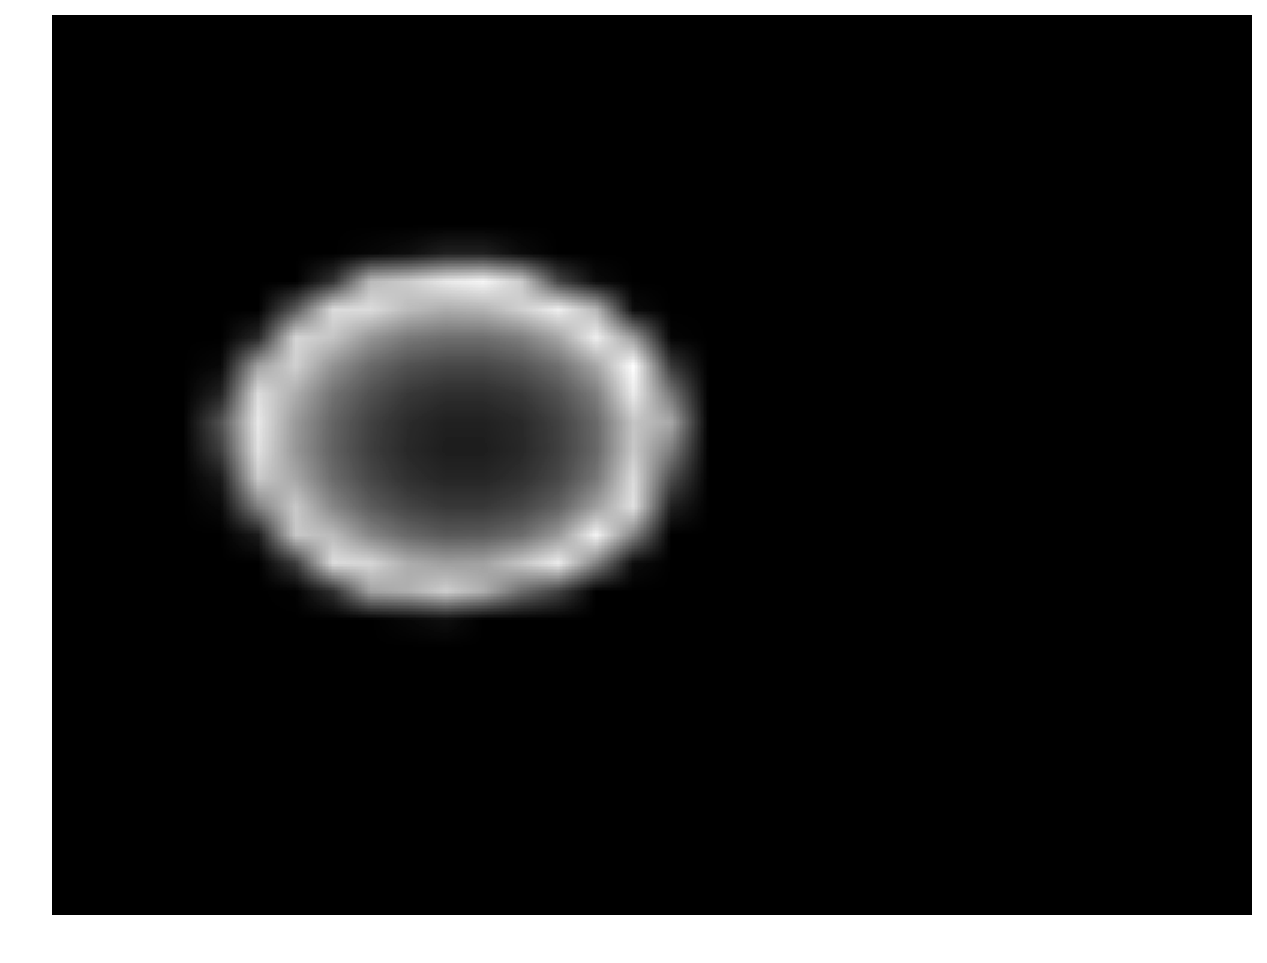
\includegraphics[width=0.75\columnwidth]{figs/depth_example.pdf} \caption{Example Depth Image} \label{fig:depth_image}
        \end{subfigure}
    \begin{subfigure}[t]{0.24\textwidth}
        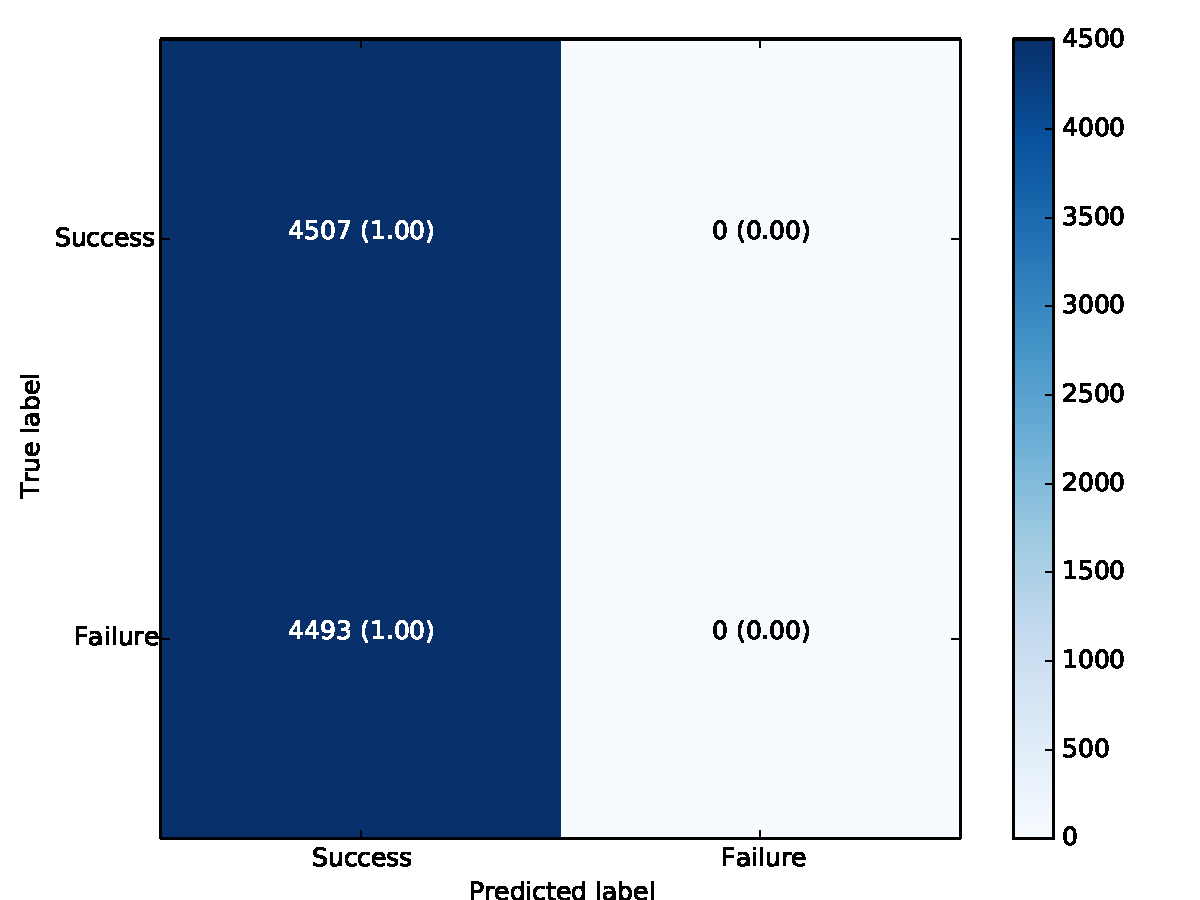
\includegraphics[width=0.9\columnwidth]{figs/balanced_results.pdf} \caption{Balanced Data} \label{fig:balanced_confusion}
    \end{subfigure}
		\begin{subfigure}[t]{0.24\textwidth}
        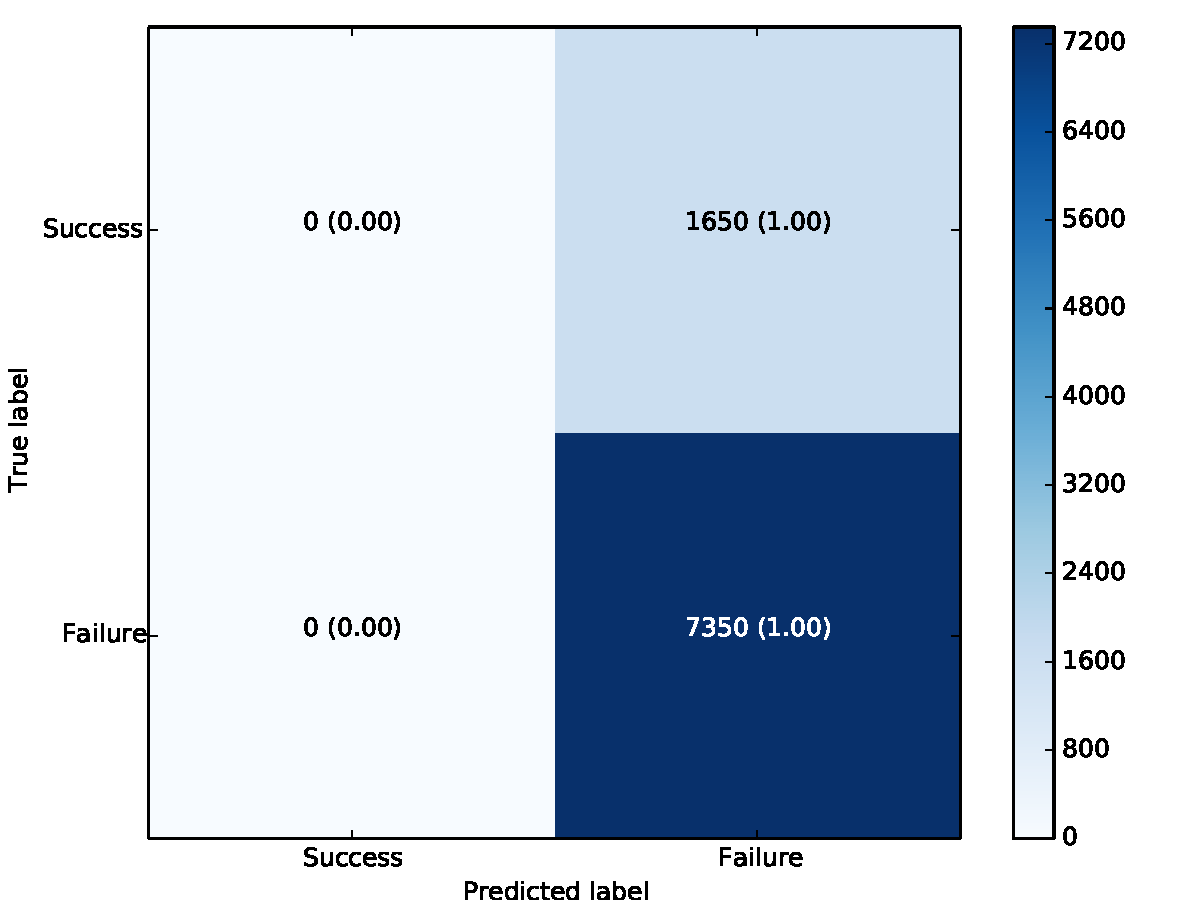
\includegraphics[width=0.9\columnwidth]{figs/unbalanced_results.pdf} \caption{Unbalanced Data} \label{fig:unbalanced_confusion}
        \end{subfigure}
    \begin{subfigure}[t]{0.24\textwidth}
        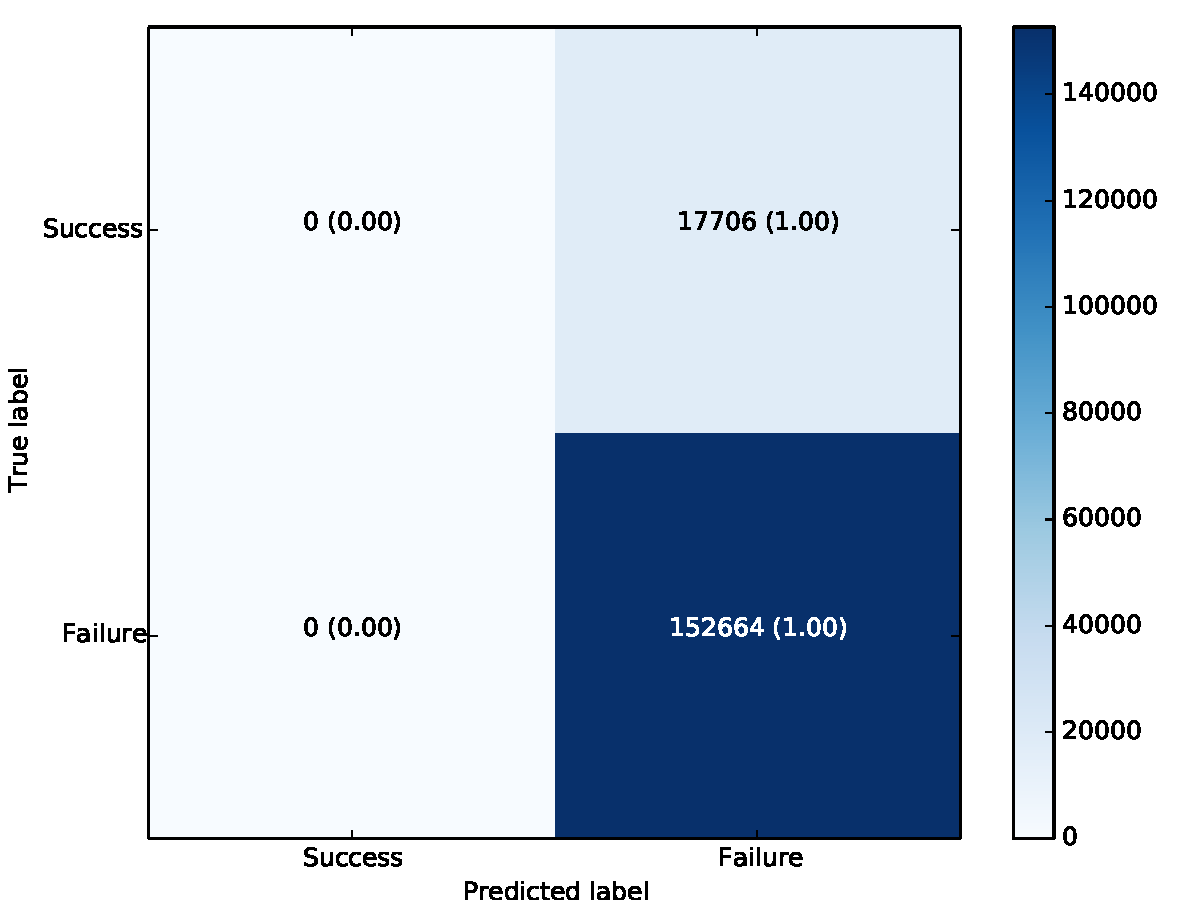
\includegraphics[width=0.9\columnwidth]{figs/paper_original.pdf} \caption{Replicated Paper Results} \label{fig:from_paper}
    \end{subfigure}
\caption{The far left panel shows a depth image that serves as input to our network. The three panels on the right show the confusion matrices for various data set learned using the pre-trained GQ-CNN network. In each case the network simply outputs, for every new instance, the label of of the largest classes. } \label{fig:confusion_matrices}
\end{figure*}

As mentioned previously, Dex-Net 2.0 contains approximately 20\% positive examples. 
Na{\"i}vely, you could predict a negative label for all instances and be correct 80\% of the time. Interesting, the paper reported an 85.7\% accuracy, which does slightly better than an all negative classifier. 

To investigate this, we begin by using their pre-trained GQ-CNN network  on the data sets we created by sampling the entire Dex Net data base. 
We can constrain our sampling to produce a data set of 10,000 samples that is 50\% positive examples and 50\% negative examples (referred to as a "balanced" data set). 
Using their network we achieve approximately 50\% accuracy because, as shown in our confusion matrix in \figref{fig:balanced_confusion}, the network learns to always output a positive label. 

If we do not make such a constraint and sample randomly, we expect to have the original distribution: 20\% positive examples and 80\% negative examples (referred to as an "unbalanced" data set). 
As shown by the confusion matrix in \figref{fig:unbalanced_confusion}, the network achieved approximately 80\% accuracy by always guessing negative. 

To confirm our thoughts a step further, we use the data they provide on their pre-trained network. 
This data set is also unbalanced and achieves similarly to above in that it always guesses negative, as seen in \figref{fig:from_paper}. 

Considering the difference between their reported results, we became suspicious of our pre-trained network~\footnote{While we cannot eliminate the possibility that we somehow loaded their network incorrectly or made a similar software implementation bug, we believe significant reasoning and debugging that we used their network correctly.}.
We therefore re-implemented their network in Keras, trained it using our balanced data set. 

Borrowing from the original paper, the network is visualized in \figref{fig:dexnet_network}. 
We briefly summarize the network structure here. 
The depth image is passed through two convolutional layers following by ReLu activation, where the convolution layers both have 64 filters and have sizes 7x7 and 5x5 respectively. 
This is followed by a max-pooling layer of size 2x2 and stride 1x1. 
This output is then passed through two more convolutional layers, where the first is following by ReLu activation, where the convolution layers both have 64 filters of size 3x3. 
We flatten this output is connect it to 1024 hidden units that are activated by a ReLu. 
The z component is connected to 20 hidden units that are activated by a ReLu and concatenated onto the result above. 
This is connected to 1024 hidden units activated by ReLU, followed by 2 hidden units. 
The softmax function is applied to give the output. 

The results from reimplemented and training GQ-CNN are shown in \figref{fig:gqcnn_results}. 
After a few time steps the training and validation accuracy achieve 60\%, which is also what our test set reported. 
The confusion matrix in \figref{fig:confusion_gqcnn}, shows our improved accuracy and that we tend to over-predict positive labels. 
As a quick note, this false positive tendency is actually more problematic for robots then false negatives, since the robot will spend time executing a grasp that is likely to fail. 

Given that the original paper reported 85\% accuracy on a data set that had approximately 80\% negative examples, our 60\% accuracy on a data set that had 50\% examples is comparable. 
However, stepping aside, a 60\% accuracy on a binary classification task leaves much to be desired. 

Hoping to improve our accuracy, we experiment with varying the architecture of the CNN. 
This both allows us to explore the effect of the architecture (as well as its hyper-parameters) and to see if we can improve upon our accuracy rate. 

\begin{figure*}[t!]
    \centering
    \begin{subfigure}[t]{0.32\textwidth}
        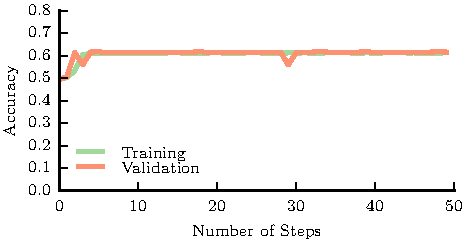
\includegraphics[width=0.9\columnwidth]{figs/gqcnn_accuracy.pdf}
        \caption{Accuracy} \label{fig:accuracy_gqcnn}
        \end{subfigure}
    \begin{subfigure}[t]{0.32\textwidth}
        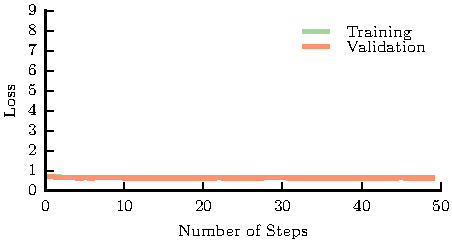
\includegraphics[width=0.9\columnwidth]{figs/gqcnn_loss.pdf}
        \caption{Loss} \label{fig:loss_qgcnn}
    \end{subfigure}
		\begin{subfigure}[t]{0.32\textwidth}
        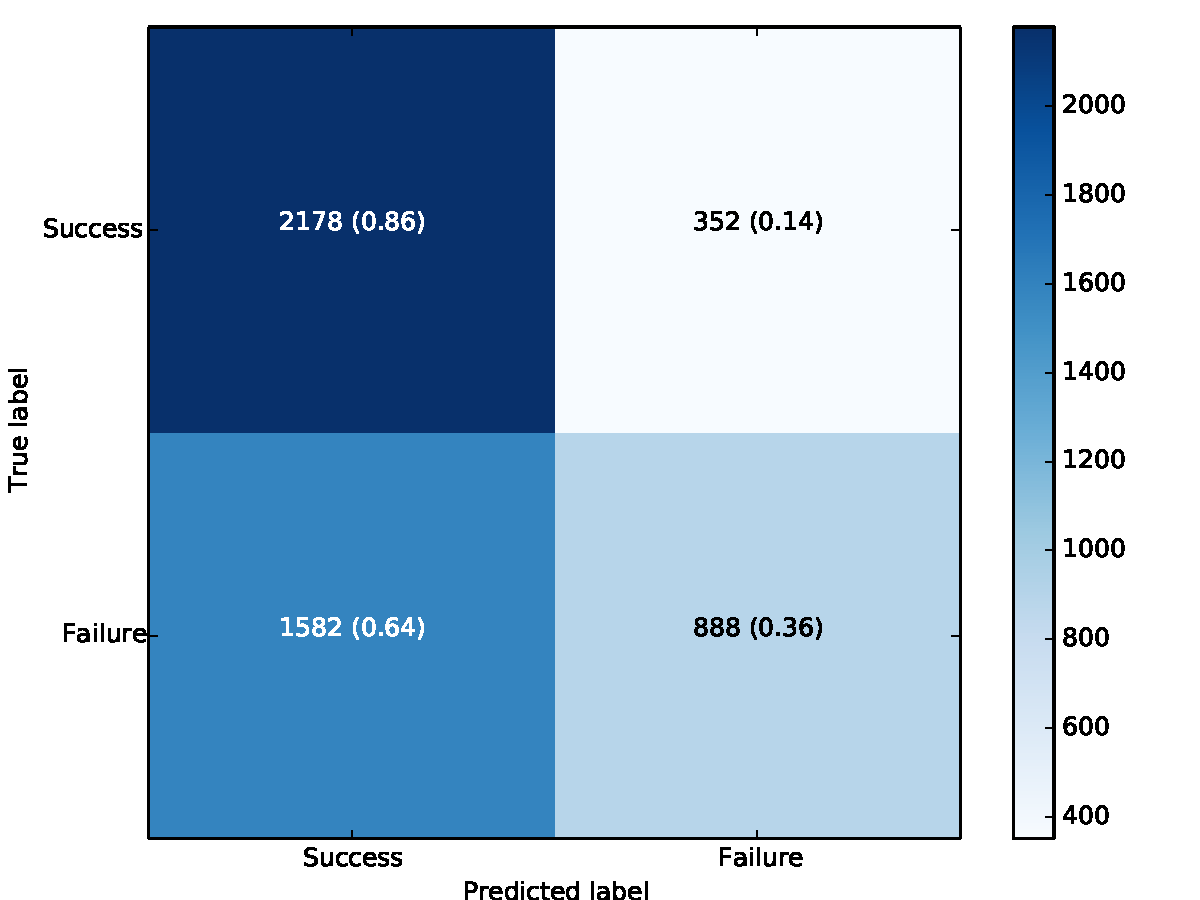
\includegraphics[width=0.8\columnwidth]{figs/trained_gqcnn.pdf}
        \caption{Confusion Matrix} \label{fig:confusion_qgcnn}
    \end{subfigure}
\caption{After re-creating and re-training the GQ-CNN network with our balanced data set, we achieve the accuracy and loss shown above on our training and validation sets. We also show the confusion matrix, as compared to the earlier results.} \label{fig:gqcnn_results}
\end{figure*}

%This result was initially surprising. 
%Due to the few percentage point disparity between our accuracy and theirs, we hesitate to conclusively claim their network did not learn features. 
%While we varied the size of the data set we use, we did not come close to their magnitude (in the millions) and therefore it is possible that the network simply needs a tremendous amount of data to learn effectively. 